\documentclass{scrartcl}
\usepackage{amsmath,amssymb,commath,graphicx,enumerate,listings}
\setkomafont{disposition}{\normalfont\bfseries}

\title{Mat 354}
\subtitle{Homework 8}
\author{Kenny Roffo}
\date{Due October 21, 2015}

\begin{document}
\maketitle

All calculations were done in R.\\

Students in a class were randomly assigned to receive one of the following two versions of a similar question:\\

\emph{Question Version A}: Suppose that you have decided to see a play for which the admission charge is \$20 per ticket. As you prepare to enter the theater, you discover that you have lost a \$20 bill. Would you still pay \$20 for a ticket to see the play?\\

\emph{Question Version B}: Suppose that you have decided to see a play and paid the admission price of \$20 per ticket. As you prepare to enter the theater, you discover that you have lost the ticket. The seat was not marked and the ticket cannot be recovered. Would you pay \$20 for another ticket?\\

Let’s assume that it makes no difference which question is asked: There are some people who will pay the \$20 to see the play, there are others who will not. (In short: Ignore for the time being the information about Questions A and B.) Suppose further that in this class of 95 students, 55 are the type who would pay the \$20 and see the play (no matter which version of question is presented): that is, 55 people will answer YES no matter what question is asked; the other 40 will answer NO. 45 students (randomly chosen from the 95) will be presented with Question Version A; the rest with Question B.

\begin{enumerate}

\item State the formula for $p(y)$, probability function for $Y = $ the number of students getting Question Version A who answer YES. List possible values for $y$.

$$p(y) = {45 \choose y}\left(\frac{55}{95}\right)^y\left(1-\frac{55}{95}\right)^{45-y}$$\\

\item Obtain the expected value, variance, and standard deviation for $Y$. (Nearest 0.01 for each.)\\

\begin{align*}
  E(Y) = \mu &= \sum_{y=5}^{45}yp(y)\\
  &= 26.05
\end{align*}

\begin{align*}
  V(Y) = \sigma^2 &= E(Y^2) - E(Y)^2\\
  &= \sum_{y=5}^{45}\left[y^2p(y)\right] - 26.05\\
  &= 10.97
\end{align*}

\begin{align*}
  SD(Y) = \sigma &= \sqrt{\sigma^2}\\
  &= 3.31
\end{align*}
\pagebreak

\item A good rule of thumb for plotting distributions is to use values $y$ that are no further than 4 standard deviations from the mean. Find the values 4 standard deviations below and above the mean (call these $l$ and $u$ respectively), then create a plot of $p(y)$ for these values.

\begin{lstlisting}[language=R]
  plot(y, p, xlim=c(l, u))
\end{lstlisting}

\begin{align*}
  l &= 12.80\\
  u &= 39.30
\end{align*}

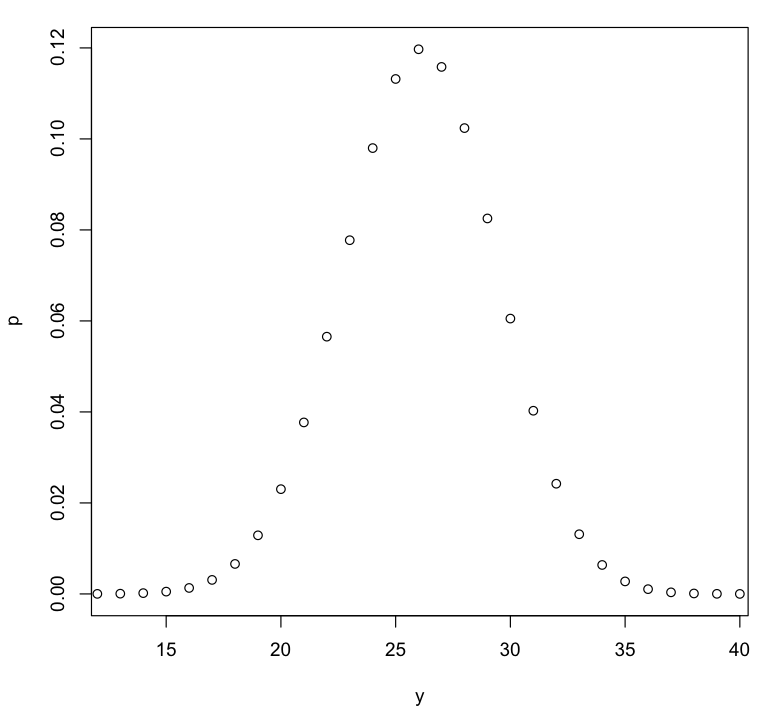
\includegraphics[keepaspectratio=true, scale=0.5]{3.png}\pagebreak

Probabilities to the nearest 0.0001 at least in what follows.

\item Determine the probability that $Y$ falls within one standard deviation of the mean (i.e. find $P(\mu – \sigma \le Y \le \mu + \sigma)$)\\

  $$\mu - \sigma = 22.7 \text{\hspace{.5in} and \hspace{.5in}}\mu + \sigma = 29.4$$

  Thus $$P(\mu – \sigma \le Y \le \mu + \sigma) = P(23 \le Y \le 29)$$ but this is just $$\sum_{y=23}^{29}p(y) = 0.7093$$

\item Determine $P(Y = 32)$ – the probability that exactly 32 of the students assigned to Question Version A answer YES.\\

  This is simply the result of plugging 32 in as the input to the function found in question 1:

\begin{align*}
  p(Y = 32) &= {45 \choose 32}\left(\frac{55}{95}\right)^32\left(1-\frac{55}{95}\right)^{45-32}\\
  &= 0.0242
\end{align*}

\item Find $P(Y \ge 32)$ – the probability that at least 32 of the students assigned to Question Version A answer YES.\\

  This is simply the result of subtracting from 1 the sum the probabilities for 5, 6, 7, ... , 30 and 31 students assigned to Question Version A answering yes.

\begin{align*}
  p(Y \ge 32) &= 1 - \left[p(Y = 5) + p(Y = 6) + ... + p(Y = 31)\right]\\
  &= 0.0480
\end{align*}
\pagebreak

The experiment is conducted and y = 32 really occurs: We’re looking at the following:

\begin{center}
\begin{tabular} { |c|c c|c| }
\hline
&Lost \$20 Bill -  QVA    Lost Ticket - QVB&Total\\
\hline
YES - Would pay to see play & 32 & & 55\\
NO - Would not pay to see play && &\\
\hline
Total & 45 && 95\\
\hline
\end{tabular}
\end{center}

\item Fill in the remaining cells of the table.

\begin{center}
\begin{tabular} { |c|c c|c| }
\hline
&Lost \$20 Bill -  QVA    Lost Ticket - QVB&Total\\
\hline
YES - Would pay to see play & 32 & 23 & 55\\
NO - Would not pay to see play & 13 & 27 & 40\\
\hline
Total & 45 & 50 & 95\\
\hline
\end{tabular}
\end{center}

\item What percentage of Question Version A answers are yes? Question Version B?\\

  Question Version A: $\frac{32}{45} = 71.1\%$\\
  Question Version B: $\frac{23}{50} = 46.0\%$\\

\item Is there a reasonable argument to be made that the nature of the situation (Question Version A vs. B) impacts (at least some) people’s choice to pay to see the play? On what basis do you form your conclusion?\\

  When losing \$20, some people feel more like they have lost money than when they have lost something worth \$20. When I buy something, I feel that I have already lost
the money spent on it. If I lose the object, I am not upset because I lost the money spent on it, but because I lost the object. In that case I won't have lost the money
unless I go buy another object. It basically comes down to the irrationality of human emotions.

\end{enumerate}
\end{document}



